\documentclass{article}
% Copyright 2022 Riley Hanus, PhD
% Unauthorized copying and use of this file, via any medium is strictly prohibited
% Proprietary and confidential
% Written by Riley Hanus <hanusriley@gmail.com>, November 2022

\usepackage[framemethod=TikZ]{mdframed} 
\usepackage{verbatim}
\usepackage{hyperref}
\usepackage{xstring}
\usepackage{listofitems}
\usepackage{substr}
\usepackage{cprotect}
% \newcounter{iframe}[chapter]\setcounter{iframe}{0}
% \renewcommand{\theiframe}{\arabic{chapter}.\arabic{iframe}}

\newenvironment{iframe}[1][]{%
% \refstepcounter{iframe}%
\ifstrempty{#1}%
{\mdfsetup{%
frametitle={%
\tikz[baseline=(current bounding box.east),outer sep=0pt]
\node[anchor=east,rectangle,fill=blue!20]
{\strut Digital Content};}}
}%
{\mdfsetup{%
frametitle={%
\tikz[baseline=(current bounding box.east),outer sep=0pt]
\node[anchor=east,rectangle,fill=blue!20]
{\strut Digital Content~:~#1};}}%
}%
\mdfsetup{innertopmargin=10pt,linecolor=blue!20,%
linewidth=2pt,topline=true,%
frametitleaboveskip=\dimexpr-\ht\strutbox\relax
}
\begin{mdframed}[]}{\end{mdframed}}

\newcommand{\parseiframe}[1]{\setsepchar{"}\readlist\iframelist{#1}
}

\newcommand{\iframeurl}[2]{
    \parseiframe{#1}
    \foreachitem \i \in \iframelist{
        \IfSubStringInString{://www.}{\i}{ \let\result=\i}{}
    }
    \href{\result}{#2}
}

\newcommand{\InsertIframe}[4]{
    % #1: html code for <iframe>
    % #2: display name for hyperlink in 'Digital Content box' in pdf
    % #3: caption
    % #4: type of media for 'Digital Content: xxx'
   \begin{iframe}[#4]
      \iframeurl{#1}{#2} | #3
   \end{iframe}
}

%%%%%%%%%%%%%%%%%%%%%%%%%%%%%%%%%%%%%%%%%%%%%%%%%%%%%%%%%%%%%%%%%%%%%%%%%%%%%%%%
% calchub environment: for embedding a calchub workspace                       %
% texedbook compatible: html=embedded work space, pdf=multimedia box w/ href   %
%%%%%%%%%%%%%%%%%%%%%%%%%%%%%%%%%%%%%%%%%%%%%%%%%%%%%%%%%%%%%%%%%%%%%%%%%%%%%%%%
\newenvironment{calchub}
    {\begin{iframe}[CalcHub Workspace]
    }
    {\end{iframe}
    }

\newcommand{\InsertCalchub}[3]{ 
   % 1st input: href 
   % 2nd input: display name
   % 3rd input: description
   \begin{calchub}
      \href{#1}{#2} | #3
   \end{calchub}
} 


%%%%%%%%%%%%%%%%%%%%%%%%%%%%%%%%%%%%%%%%%%%%%%%%%%%%%%%%%%%%%%%%%%%%%%%%%%%%%%%%
% video environment: for embedding videos                                      %
% texedbook compatible: html=embedded video, pdf=multimedia box w/ href        %
%%%%%%%%%%%%%%%%%%%%%%%%%%%%%%%%%%%%%%%%%%%%%%%%%%%%%%%%%%%%%%%%%%%%%%%%%%%%%%%%
\newenvironment{youtube}
   {\begin{iframe}[Video]
   }
   {\end{iframe}
   }

\newcommand{\InsertYouTube}[3]{ 
   % 1st input: href   
   % 2nd input: display name 
   % 3rd input: description
   \begin{youtube}
      \href{#1}{#2} | #3
   \end{youtube}
} 

%%%%%%%%%%%%%%%%%%%%%%%%%%%%%%%%%%%%%%%%%%%%%%%%%%%%%%%%%%%%%%%%%%%%%%%%%%%%%%%%
% python coding environment: for coding practice                               %
% texedbook compatible: html=embedded trinket, pdf=multimedia box w/ href      %
%%%%%%%%%%%%%%%%%%%%%%%%%%%%%%%%%%%%%%%%%%%%%%%%%%%%%%%%%%%%%%%%%%%%%%%%%%%%%%%%


\newenvironment{trinket}
   {\begin{iframe}[Python coding environment]
   }
   {\end{iframe}
   }

\newcommand{\InsertTrinket}[3]{ 
   % 1st input: href   
   % 2nd input: display name 
   % 3rd input: description
   \begin{trinket}
      \href{#1}{#2} | {#3}
   \end{trinket}
} 


%%%%%%%%%%%%%%%%%%%%%%%%%%%%%%%%%%%%%%%%%%%%%%%%%%%%%%%%%%%%%%%%%%%%%%%%%%%%%%%%
% panopto environment: for viewing videos hosted by panopto                    %
% texedbook compatible: html=embedded iframe, pdf=multimedia box w/ href       %
%%%%%%%%%%%%%%%%%%%%%%%%%%%%%%%%%%%%%%%%%%%%%%%%%%%%%%%%%%%%%%%%%%%%%%%%%%%%%%%%


\newenvironment{panopto}
   {\begin{iframe}[Video]
   }
   {\end{iframe}
   }

\newcommand{\InsertPanoptoVideo}[3]{ 
   % 1st input: href   
   % 2nd input: display name 
   % 3rd input: description
   \begin{panopto}
      \href{#1}{#2} | {#3}
   \end{panopto}
} 

% Mathjax equation referencing
\newcommand\mjref[1]{\ref{#1}}


\usepackage{hyperref}
\usepackage{verbatim}

\title{Author's guide to texedbook}
\author{Riley Hanus}

\begin{document}
 
\maketitle

\begin{abstract}
\noindent The \verb'texedbook' code base is a tool for publishing articles and textbooks online without the need to learn html, css, and javascript. The author writes and compiles the content in latex and (after following the set-up instructions in the README.md) runs 
\begin{verbatim}
python run.py ./path/to/latex/project/directory
\end{verbatim}
which generates a collection of html and css files that can be directly published online. The product is a computer and mobile friendly webpage,  In addition to supporting most of the native latex features, texedbook provides tools for embedding digital and interactive content such as videos, quizzes, code editors and compilers, etc. 

\noindent This article acts as an author's guide to \verb'texedbook' and will demonstrate the document features that are explicitly supported, and the specific way they must be used for a clean output html page.  First, the native latex capabilities will be demonstrated including figures, equations, tables, cross-referencing, citations, etc. Then the \verb'texedbook' specific features will be presented which allow the author to embed digital content (essentially anything that can be contained in an iframe) straight from the latex document. 
\end{abstract}

\section{Motivation for texedbook project}

When writing an article or textbook, especially one that is technical in nature, the need for proper handling of standard document features is glaring. Without a framework to efficiently manage citations, cross-reference document items (sections, equations, figures, etc.), and write math in real time, writing anything with technical substance becomes prohibitively difficult. Latex, despite its quarks, is a very good framework to manage these critical writing tools and compiling beautifully typeset pdf documents.

At the same time, publishing and education has transitioned to digital-first for the consumer, yet publishers still cling to a print-first model. There is a clear need for a tool enabling authors to publish digital-first articles, books, and courses. The natural medium this digital-first publishing is an html/css/js based webpage. 

\verb'texedbook' combines the strengths of latex for authoring articles and books with the versatility and universality of an html/css/js based webpage.  

\section{Native latex features} \label{sec:latexfeatures}
\subsection{Figures}
All figures used in the document must be contained in a directory named \verb'./figures/' and that folder must be located in the same location as \verb'main.tex'. In addition, all figures must be in pdf format.

Ensuring that the figures are displayed correctly in the resulting html is tricky. The simplest and most effective way is to design the width of all figures to span width of the text on the page. This display condition reliably converts from latex to html and translates from computer to mobile formats well, which is not the case for all display options. If you would like the figure to display smaller, simply add white space to the left and right of the pdf as is done in Figure \ref{fig:example}.

An example of the latex code used to add a figure is
\begin{verbatim}
    \begin{figure}[t]
        \centering
        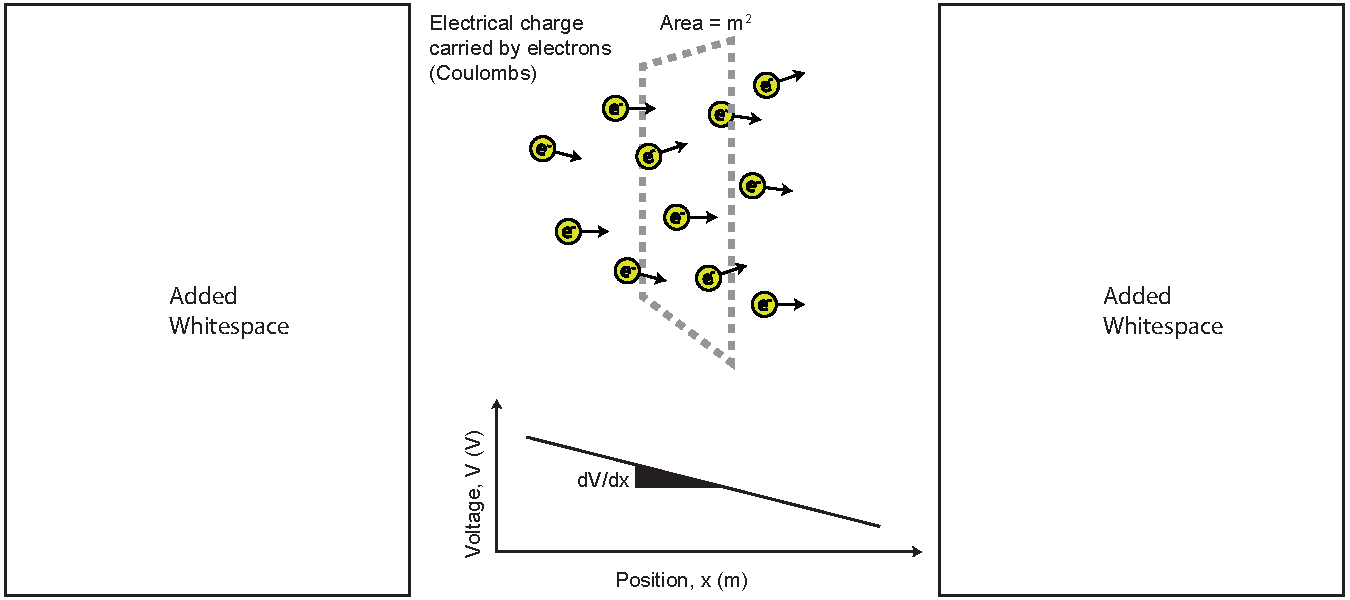
\includegraphics[width=0.99\textwidth, keepaspectratio]{figures/fig.pdf}
        \caption{Example figure. Since the convention for texedbook is for figures to span the text width, whitespace added to control size of the image.}
        \label{fig:example}
    \end{figure}  
\end{verbatim}
The [t] places the figure at the top of a page in the pdf, and does nothing to the html output. The html output will place the figure where it appears in the code.

\begin{figure}[t]
    \centering
    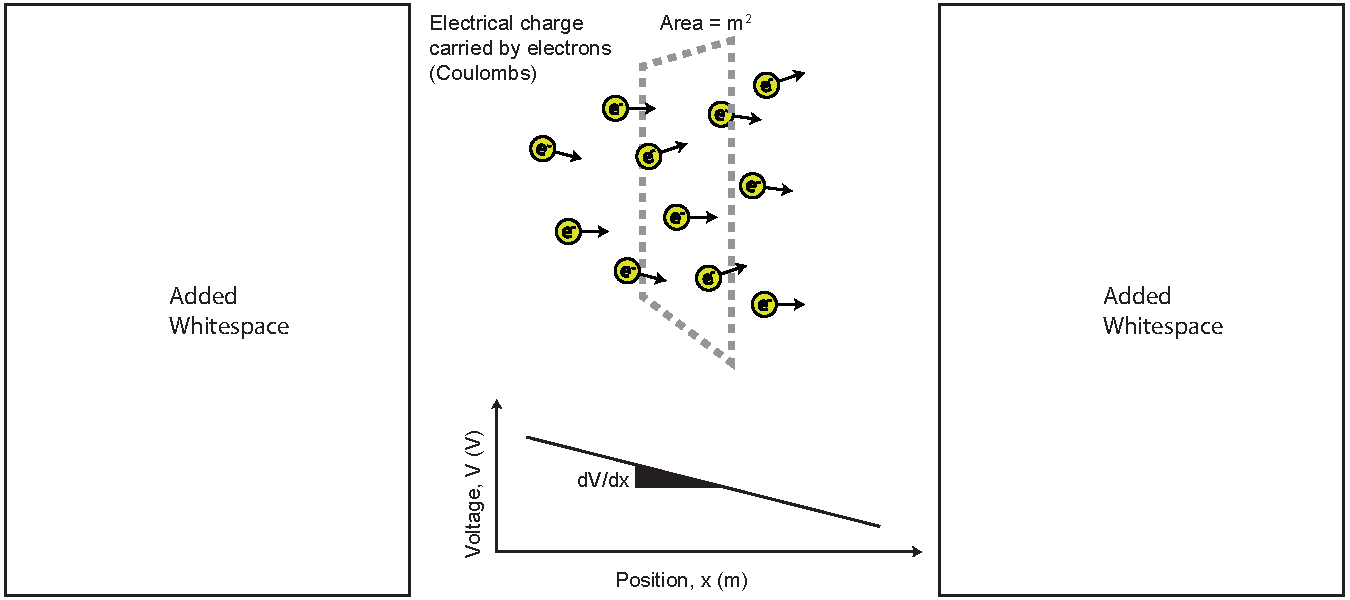
\includegraphics[width=0.99\textwidth, keepaspectratio]{figures/fig.pdf}
    \caption{Example figure. Since the convention for texedbook is for figures to span the text width, whitespace added to control size of the image.}
    \label{fig:example}
\end{figure}



\subsection{Equations} \label{sec:equations}
Equations are an inherently tricky problem for digital publishing. The core of the problem lies in the fact that html was designed around the standard alphanumeric alphabet, and math requires a wider range of complex symbols and typesetting. The default usage of \verb'texedbook' leverages \verb'mathjax', allowing all the native latex equations to be reliably reproduced in the html output.

In line equations can be included $n\lambda=2d \sin \theta$, as well as displayed equations 
\begin{equation}
    n\lambda=2d \sin \theta.
    \label{eq:braggslaw}
\end{equation}
Cross-referencing equations is done using the \verb'\mjref' function provided in \verb'texedbook.tex'. For example, Eq. \mjref{eq:braggslaw} is Bragg's Law, commonly used to find diffraction conditions of light of wavelength $\lambda$ interacting with a crystal with lattice spacing $d$ at an incident angle of $\theta$. The \verb'\mjref' function simply substitutes \verb'\ref' when the latex is compiled. However, when \verb'tex4ebook' converts the project to html, \verb'config.cfg' file tells \verb'tex4ebook' to insert \verb'\eqref' in place of all \verb'\mjref's, which \verb'mathjax' knows to look for in the html and use for equation numbering and cross-referencing. 

\subsection{Tables}
Tables are inherently difficult to write in latex. \href{https://www.tablesgenerator.com/}{Tables Generator} is a great tool for generating latex code for tables. The table is translated into html. Note that the table styling in the html output is different than the latex output. 

\begin{table}[]
    \caption{Example table.}
    \label{table:example}
    \centering
    \begin{tabular}{|c|c|c|c|}
    \hline
    \multicolumn{1}{|l|}{Sample} & \multicolumn{1}{l|}{Data 1} & \multicolumn{1}{l|}{Data  2} & \multicolumn{1}{l|}{Data 3} \\ \hline
    A                            & 53                          & 62                           & 75                          \\ \hline
    B                            & 51                          & 61                           & 72                          \\ \hline
    C                            & 58                          & 69                           & 71                          \\ \hline
    \end{tabular}
    \end{table}

\subsection{Code}
Code can be displayed using the verbatim environment native to latex 
\begin{verbatim}
\begin{verbatim}
    for i in list:
        i='some code'
\end{verb atim} 
\end{verbatim}

Code can be written in-line using the \verb'\verb' function. This function comes from the \verb'verbatim' package and is unique in that it doesn't use the curly brackets for its arguement. It takes the first non-letter character as the open arguement and looks for that same character again to close the arguement. I typically use \verb_\verb'code here'_.   


\subsection{Cross-referencing and hyperlinks}
Cross-referencing can be used as normal in latex and all of the hyperlinking functionality will be preserved in the html. For example, Section \ref{sec:latexfeatures}, Table \ref{table:example}, and Figure \ref{fig:example}. The only important exception is Equations where the \verb'\mjref' command must be used such that mathjax can properly lable and cross-reference equations locally in the html page using javascript (see Section \ref{sec:equations}).

Hyperlinks to external webpages can be added in latex using the \verb'\href' command.
\begin{verbatim}
    \href{https://www.webpage.com}{Display name in document}
\end{verbatim}

\subsection{Citations}
The native bibliography features are maintained. For example, one can cite an article \cite{Hanus2021} or multiple articles \cite{Hanus2019,Hanus2021,Gregory2021}. Note that the hyperlinking to the bibliography in the pdf, a result of using the \verb'hyperref' package, is maintained in the resulting html. The default bibliography style used in \verb'texedbook' is \verb'unsrturl'. Note that this style supports hyperlinking to the url, and/or doi if that field is present in the .bib entry, and the hyperlinking is maintained in the resulting html. It is recommended that the doi field is used instead of the url, since line breaking needed to typset urls is handeled poorly by latex. Latex's performance on typesetting doi hyperlinks seems to work more reliably.

\bibliographystyle{unsrturl}
\bibliography{sample}

\end{document}

